\documentclass{article} % For LaTeX2e
\usepackage{float}
\usepackage{nips13submit_e,times}
\usepackage{hyperref}
\usepackage{url}
\usepackage{graphicx}
\usepackage{kotex}
\usepackage[sorting=none]{biblatex}
\addbibresource{ee531.bib}
\usepackage{amssymb}
\usepackage{amsthm}

\newtheorem{theorem}{Theorem}
\newtheorem{proposition}{Proposition}

\theoremstyle{definition}
\newtheorem{definition}{Definition}
\newtheorem{algorithm}{Algorithm}
\title{EE531 Project Proposal (Team 5)}


% The \author macro works with any number of authors. There are two commands
% used to separate the names and addresses of multiple authors: \And and \AND.
%
% Using \And between authors leaves it to \LaTeX{} to determine where to break
% the lines. Using \AND forces a linebreak at that point. So, if \LaTeX{}
% puts 3 of 4 authors names on the first line, and the last on the second
% line, try using \AND instead of \And before the third author name.

\newcommand{\fix}{\marginpar{FIX}}
\newcommand{\new}{\marginpar{NEW}}

%\nipsfinalcopy % Uncomment for camera-ready version

\begin{document}


\maketitle

\begin{abstract}
This project will be a \textbf{Generative Adversarial Network} (GAN) review. It includes paper review, implementation of recent GAN.
\end{abstract}

\section{Topic review: Generative Adversarial Network}
\textbf{Generative Adversarial Network} (GAN) is a new framework \cite{goodfellow2014generative} for estimating generative models via an adversarial process trained simultaneously. This framework corresponds to a \textbf{minimax two-player game}. There are two models for training simultaneously: a generative model \textit{G} that captures the data distribution, and a discriminative model \textit{D} that estimates the probability that a sample came from the training data rather than \textit{G}. The training procedure for \textit{G} is to maximize the probability of \textit{D} making a mistake. 

\subsection{Adversarial nets}

The adversarial modeling framework is most straightforward to apply when the models are both multilayer perceptrons. 

\begin{definition}
To learn the generator's distribution $p_g$ over the data $\textbf{x}$, let a prior on input noise variables be $p_\textbf{z}(\textbf{z})$ and represent a mapping to data space as $G(\textbf{z};\theta_g)$, where $G$ is a differentiable function represented by a multilayer perceptron with parameter $\theta_g$.
\end{definition}

\begin{definition}
Let a second multilayer perceptron $D(\textbf{x};\theta_d)$ that outputs a single scalar. $D(\textbf{x})$ represents the probability that $\textbf{x}$ came from the data rather than $p_g$.
\end{definition}

Then $D$ and $G$ play the following two-player minimax game with value function $V(G,D)$:
\begin{equation}
    \min_G\max_D V(D,G) = \mathbb{E}_{\textbf{x} \sim p_{data}(\textbf{x})}[\log D(\textbf{x})] + \mathbb{E}_{\textbf{z}\sim p_\textbf{z}(\textbf{z})}[\log(1-D(G(\textbf{z})))]
\label{eq:valuefunction}
\end{equation}

In other words, $D$ is trained to maximize the probability of assigning the correct label to both training examples and samples from $G$. Simultaneously, G is trained to minimize $\log(1-D(G(\textbf{z})))$.

\begin{algorithm}
Minibatch stochastic gradient descent training of generative adversarial nets. The number of steps to apply to the discriminator, $k$, is a hyperparameter. $k=1$ in experiments
\begin{figure}[H]
	\centering
	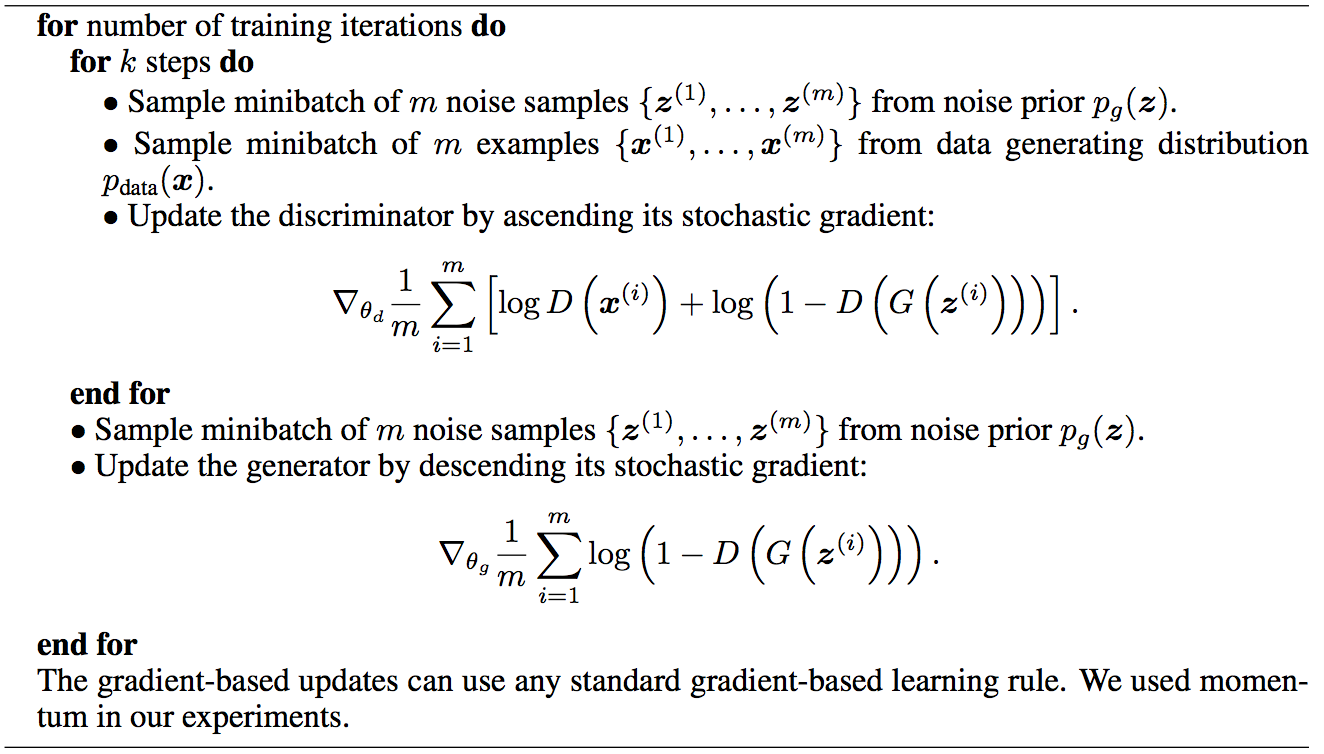
\includegraphics[width=0.9\linewidth]{2}
	\label{fig:algo}
\end{figure}
\end{algorithm}
\subsection{Explanation of this approach}
Figure \ref{fig:gan1}: Generative adversarial nets are trained by simultaneously updating the \textbf{discriminative} distribution ($D$, blue, dashed line) so that it discriminates between samples from the data generating distribution (black, dotted line) $p_x$ from those of the \textbf{generative} distribution $p_g(G)$ (green,solid line). The lower horizontal line is the domain from which $\textbf{z}$ is sampled, in this case uniformly. The horizontal line above is part of the domain of $\textbf{x}$. The upward arrows show how the mapping $\textbf{x}=G(\textbf{x})$ imposes the non-uniform distribution $p_g$ on transformed samples. $G$ contracts in regions of high density and expands in regions of low density of $p_g$. (a) Consider an adversarial pair near convergence: $p_g$ is similar to $p_{data}$ and $D$ is a partially accurate classifier. (b) In the inner loop of the algorithm $D$ is trained to discriminate samples from data, converging to $D^*(\textbf{x})=\frac{p_{data}(x)}{p_{data}(x)+p_g(x)}$. (c) After an update to $G$, gradient of $D$ has guided $G(\textbf{z})$ to flow to regions that are more likely to be classified as data. (d) After several steps of training, if $G$ and $D$ have enough capacity, they will reach a point at which both cannot improve because $p_g = p_{data}$. The discriminator is unable to differentiate between the two distributions, i.e. $D(\textbf{x}) = \frac{1}{2}$.
\begin{figure}[H]
	\centering
	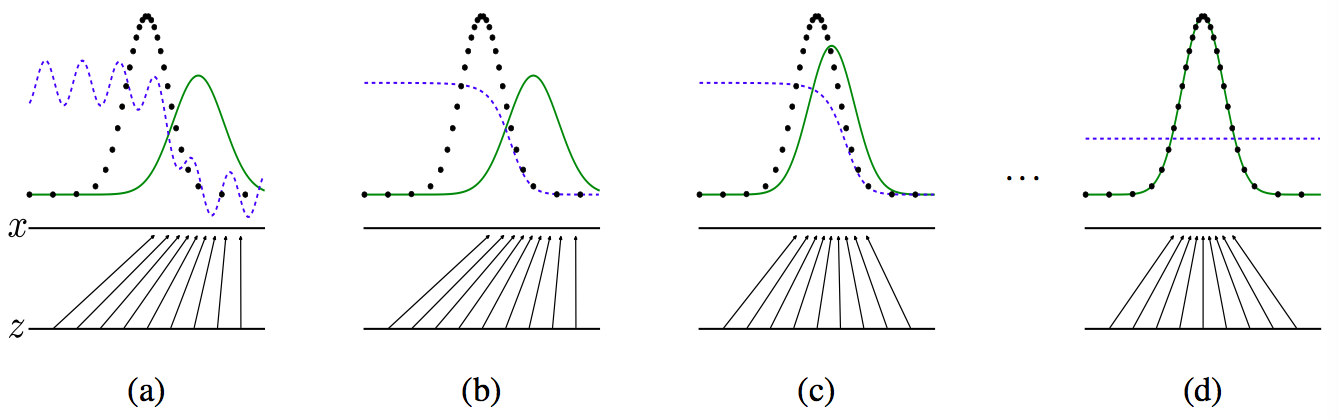
\includegraphics[width=0.9\linewidth]{1}
	\caption{Example}
	\label{fig:gan1}
\end{figure}

\subsection{Global optimality of $p_g = p_{data}$}

\begin{proposition}
For $G$ fixed, the optimal discriminator $D$ is
\begin{equation}
    D_G^*(\textbf{x}) = \frac{p_{data}(\textbf{x})}{p_{data}(\textbf{x})+p_g(\textbf{x})}
\label{eq:prop1}
\end{equation}
\end{proposition}

\begin{proof}
The training criterion for the discriminator $D$, given any generator $G$, is to maximize the quantity $V(G,D)$
\begin{eqnarray}
    V(G,D) &=& \int_{\textbf{x}}{p_{data}(\textbf{x})\log(D(\textbf{x}))dx} + \int_\textbf{z}{p_\textbf{z}(\textbf{z})\log(1-D(g(\textbf{z})))dz} \nonumber \\
    &=& \int_\textbf{x}{p_{data}(\textbf{x})\log(D(\textbf{x}))+p_g(\textbf{x})\log(1-D(\textbf{x}))dx} \nonumber
\end{eqnarray}
For any $(a,b)\in \mathbb{R}^2\setminus{0,0}$, the function $y \rightarrow a\log(y) + b\log(1-y)$ achieves its maximum in $[0,1]$ at $\frac{a}{a+b}$. The discriminator does not need to be defined outside of $Supp(p_{data}) \cup Supp(p_g)$, concluding the proof.
\end{proof}

Note that the training objective for $D$ can be interpreted as maximizing the log-likelihood for estimating the conditional probability $P(Y - y\mid\textbf{x})$, where $Y$ indicates whether $\textbf{x}$ comes from $p_{data}$ (with $y=1$) or from $p_g$ (with $y=0$). The minimax game in Eq.\ref{eq:valuefunction} can now be reformulated as: 
\begin{eqnarray}
    C(G) &=& \max_D V(G,D) \nonumber \\
    &=& \mathbb{E}_{\textbf{x}\sim p_{data}}[\log D_G^*(\textbf{x})] + \mathbb{E}_{\textbf{z} \sim p_\textbf{z}}[\log (1-D_G^*(G(\textbf{z})))] \nonumber \\
    &=& \mathbb{E}_{\textbf{x}\sim p_{data}}[\log D_G^*(\textbf{x})] + \mathbb{E}_{\textbf{z} \sim p_g}[\log (1-D_G^*(\textbf{x})] \nonumber \\
    &=& \mathbb{E}_{\textbf{x}\sim p_{data}}[\log \frac{p_{data}(\textbf{x})}{p_{data}(\textbf{x})+p_{g}(\textbf{x})}] + \mathbb{E}_{\textbf{x}\sim p_{g}}[\log \frac{p_{g}(\textbf{x})}{p_{data}(\textbf{x})+p_{g}(\textbf{x})}]
    \label{eq:4}
\end{eqnarray}

\begin{theorem}
The global minimum of the virtual training criterion $C(G)$ is achieved if and only if $p_g=p_{data}$. At that point, $C(G)$ achieves the value $-\log4$.
\end{theorem}
\begin{proof}
For $p_g=p_{data}$, $D_G^*(\textbf{x})=\frac{1}{2}$, (consider Eq. \ref{eq:prop1}). Hence, by inspecting Eq. \ref{eq:4} at $D_G^*(\textbf{x})=\frac{1}{2}$, we find $C(G) = \log \frac{1}{2} +\log \frac{1}{2} = -\log4$. To see that this is the best possible value of $C(G)$, reached only for $p_g=p_{data}$, observe that
\begin{equation}
    \mathbb{E}_{\textbf{x}\sim p_{data}}[-\log2]+\mathbb{E}_{\textbf{x}\sim p_{g}}[-\log2]=-\log4
\end{equation}
and that by subtracting this expression from $C(G) = V(D_G^*,G)$, we obtain:
\begin{equation}
    C(G) = -\log4 + KL(p_{data} \parallel \frac{p_{data}+p_{g}}{2}) + KL(p_{g} \parallel \frac{p_{data}+p_{g}}{2})
\end{equation}
where KL is the Kullback-Leibler divergence. We recognize in the previous expression the Jensen-Shannon divergence between the model's distribution and the data generating process:
\begin{equation}
    C(G) = -\log4 + 2\dot JSD(p_{data} \parallel p_{g})
\end{equation}
Since the Jensen-Shannon divergence between two distributions is always non-negative, and zero iff they are equal, we have shown that $C^*=-\log4$ is the global minimum of $C(G)$ and that the only solution is $p_g=p_{data}$, i.e., the generative model perfectly replicating the data distribution.
\end{proof}

\subsection{Convergence of Algorithm 1}
\begin{proposition}
If $G$ and $D$ have enough capacity, and at each step of Algorithm 1, the discriminator is allowed to reach its optimum given $G$, and $p_g$ is updated so as to improve the criterion
\begin{equation}
    \mathbb{E}_{\textbf{x}\sim p_{data}}[\log D_G^*(\textbf{x})] + \mathbb{E}_{\textbf{z} \sim p_g}[\log (1-D_G^*(\textbf{x})]
\end{equation}
then $p_g$ converges to $p_{data}$
\end{proposition}

\section{Project objective}
\subsection{Plan}
\begin{itemize}
    \item Explaination of GAN
    \item Proof of GAN's properties: $\exists$ unique solution and convergence of GAN
    \item Related works flow
    \item Implementation of GAN
\end{itemize}

\subsection{Related works of GAN}

\begin{itemize}
    \item On Discriminative vs. Generative classifiers: A comparison of logistic regression and naive Bayes (NIPS'02) \cite{disc}
    \item Deep Boltzmann machine \cite{salakhutdinov2009deep}
    \item Generative stochastic networks \cite{bengio2014deep}
    \item Improvement of GAN \cite{SalimansGZCRC16}
    \item Laplacian Pyramid GAN (NIPS'16) \cite{denton2015deep}
    \item Info GAN, which is unsupervised training \cite{ChenDHSSA16}
    \item DCGAN (ICLR'16) \cite{radford2015unsupervised}
    \item Semantic image inpainting \cite{yeh2016semantic}
    \item BEGAN: Boundary Equilibrium Generative Adversarial Networks (2017) \cite{berthelot2017began}
    \item Energy-based GAN (ICLR'17) \cite{zhao2016energy}
    \item Grayscale image colorization \cite{cao2017unsupervised}
\end{itemize}

\subsection {Implement of GAN}
It will be implemented the \textbf{recently significant GAN} structure. I will exclude as much as possible GAN papers whose implementation has already been opened. Environment: Tensorflow (GTX970)
\printbibliography
\end{document}
